\documentclass{standalone}
\usepackage{tikz}
\usetikzlibrary{patterns, positioning}

\begin{document}
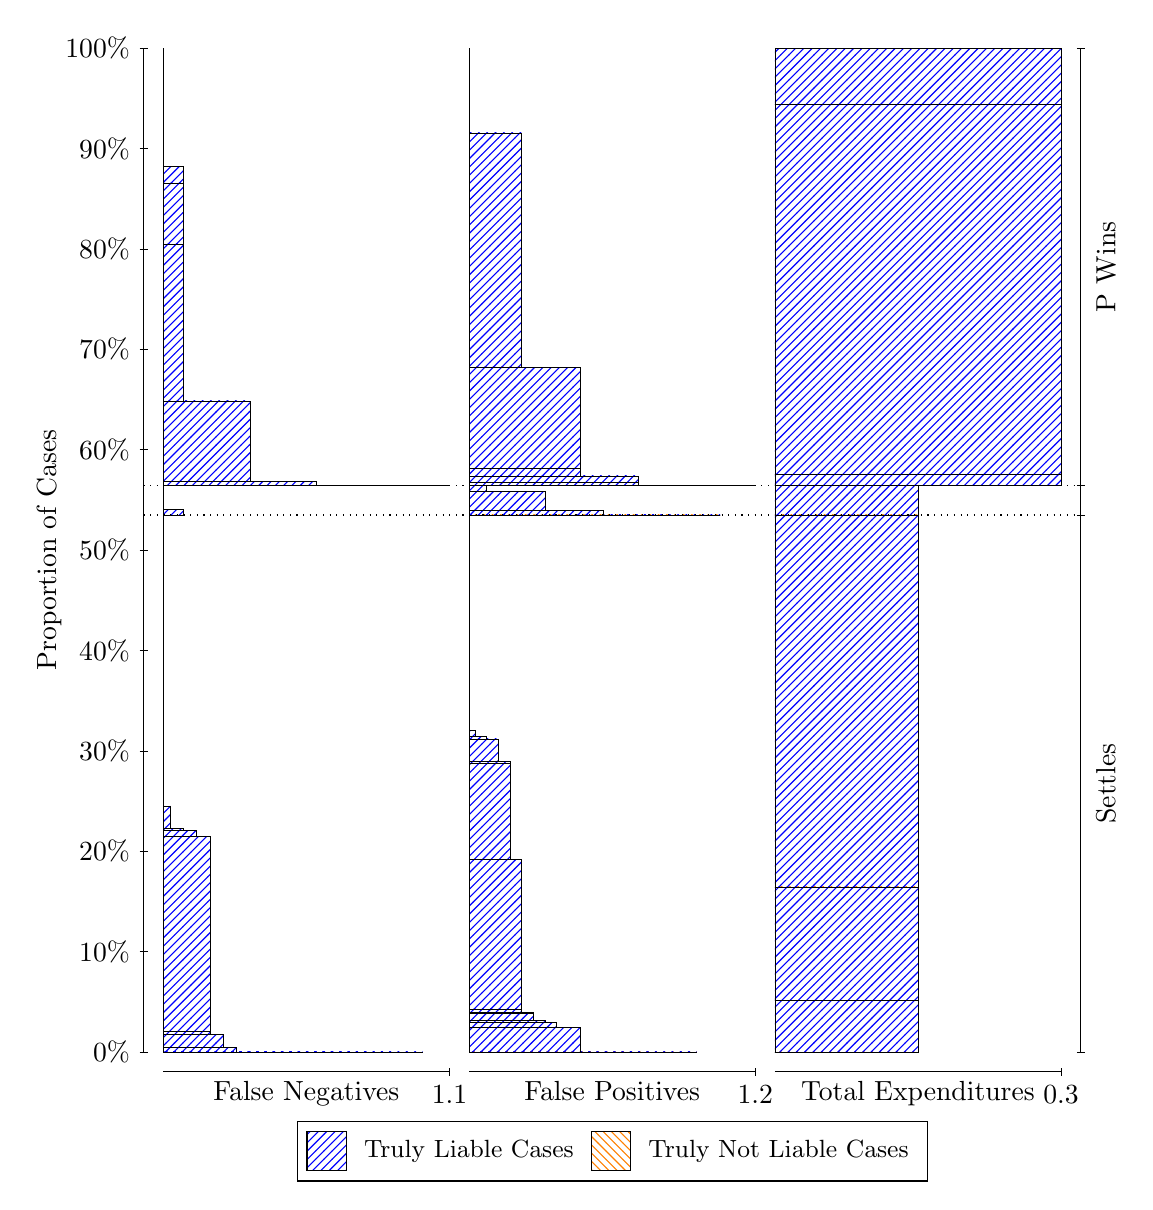
\begin{tikzpicture}
\draw[black, very thin] (1.5,1.75) -- (1.5,14.5);
\node[rotate=90, anchor=center] at (0.3, 8.125) {Proportion of Cases};
\draw[black, very thin] (1.45,1.75) -- (1.55,1.75);
\node[anchor=east] at (1.45, 1.75) {0\%};
\draw[black, very thin] (1.45,3.025) -- (1.55,3.025);
\node[anchor=east] at (1.45, 3.025) {10\%};
\draw[black, very thin] (1.45,4.3) -- (1.55,4.3);
\node[anchor=east] at (1.45, 4.3) {20\%};
\draw[black, very thin] (1.45,5.575) -- (1.55,5.575);
\node[anchor=east] at (1.45, 5.575) {30\%};
\draw[black, very thin] (1.45,6.85) -- (1.55,6.85);
\node[anchor=east] at (1.45, 6.85) {40\%};
\draw[black, very thin] (1.45,8.125) -- (1.55,8.125);
\node[anchor=east] at (1.45, 8.125) {50\%};
\draw[black, very thin] (1.45,9.4) -- (1.55,9.4);
\node[anchor=east] at (1.45, 9.4) {60\%};
\draw[black, very thin] (1.45,10.675) -- (1.55,10.675);
\node[anchor=east] at (1.45, 10.675) {70\%};
\draw[black, very thin] (1.45,11.95) -- (1.55,11.95);
\node[anchor=east] at (1.45, 11.95) {80\%};
\draw[black, very thin] (1.45,13.225) -- (1.55,13.225);
\node[anchor=east] at (1.45, 13.225) {90\%};
\draw[black, very thin] (1.45,14.5) -- (1.55,14.5);
\node[anchor=east] at (1.45, 14.5) {100\%};

\draw[black, very thin] (13.4,1.75) -- (13.4,14.5);
\draw[black, very thin] (13.35,1.75) -- (13.45,1.75);
\node[anchor=west] at (13.35, 1.75) {};
\draw[black, very thin] (13.35,8.57) -- (13.45,8.57);
\node[anchor=west] at (13.35, 8.57) {};
\draw[black, very thin] (13.35,8.941) -- (13.45,8.941);
\node[anchor=west] at (13.35, 8.941) {};
\draw[black, very thin] (13.35,14.5) -- (13.45,14.5);
\node[anchor=west] at (13.35, 14.5) {};

\draw[black, very thin, pattern color=blue, pattern=north east lines] (1.75,1.75) rectangle (5.0453,1.75);
\draw[black, very thin, pattern color=blue, pattern=north east lines] (1.75,1.75) rectangle (4.7074,1.75);
\draw[black, very thin, pattern color=blue, pattern=north east lines] (1.75,1.75) rectangle (4.3694,1.75);
\draw[black, very thin, pattern color=blue, pattern=north east lines] (1.75,1.75) rectangle (4.2004,1.75);
\draw[black, very thin, pattern color=blue, pattern=north east lines] (1.75,1.75) rectangle (4.0314,1.75);
\draw[black, very thin, pattern color=blue, pattern=north east lines] (1.75,1.75) rectangle (3.8624,1.75);
\draw[black, very thin, pattern color=blue, pattern=north east lines] (1.75,1.75) rectangle (3.6934,1.75);
\draw[black, very thin, pattern color=blue, pattern=north east lines] (1.75,1.75) rectangle (3.5244,1.7501);
\draw[black, very thin, pattern color=blue, pattern=north east lines] (1.75,1.7501) rectangle (3.3554,1.7508);
\draw[black, very thin, pattern color=blue, pattern=north east lines] (1.75,1.7508) rectangle (3.1864,1.7508);
\draw[black, very thin, pattern color=blue, pattern=north east lines] (1.75,1.7508) rectangle (3.1864,1.7509);
\draw[black, very thin, pattern color=blue, pattern=north east lines] (1.75,1.7509) rectangle (3.0174,1.7517);
\draw[black, very thin, pattern color=blue, pattern=north east lines] (1.75,1.7517) rectangle (2.8484,1.7518);
\draw[black, very thin, pattern color=blue, pattern=north east lines] (1.75,1.7518) rectangle (2.6795,1.8081);
\draw[black, very thin, pattern color=blue, pattern=north east lines] (1.75,1.8081) rectangle (2.5105,1.9737);
\draw[black, very thin, pattern color=blue, pattern=north east lines] (1.75,1.9737) rectangle (2.3415,1.9737);
\draw[black, very thin, pattern color=blue, pattern=north east lines] (1.75,1.9737) rectangle (2.3415,2.0089);
\draw[black, very thin, pattern color=blue, pattern=north east lines] (1.75,2.0089) rectangle (2.3415,4.4864);
\draw[black, very thin, pattern color=blue, pattern=north east lines] (1.75,4.4864) rectangle (2.1725,4.5664);
\draw[black, very thin, pattern color=blue, pattern=north east lines] (1.75,4.5664) rectangle (2.0035,4.5927);
\draw[black, very thin, pattern color=blue, pattern=north east lines] (1.75,4.5927) rectangle (1.8345,4.8766);
\draw[black, very thin, pattern color=orange, pattern=north west lines] (1.75,4.8766) rectangle (1.75,4.8766);
\draw[black, very thin, pattern color=blue, pattern=north east lines] (1.75,4.8766) rectangle (1.75,8.57);
\draw[black, very thin, pattern color=blue, pattern=north east lines] (1.75,8.57) rectangle (2.0035,8.6383);
\draw[black, very thin, pattern color=orange, pattern=north west lines] (1.75,8.6383) rectangle (1.75,8.6383);
\draw[black, very thin, pattern color=blue, pattern=north east lines] (1.75,8.6383) rectangle (1.75,8.941);
\draw[black, very thin, pattern color=blue, pattern=north east lines] (1.75,8.941) rectangle (5.3833,8.941);
\draw[black, very thin, pattern color=blue, pattern=north east lines] (1.75,8.941) rectangle (4.5384,8.9412);
\draw[black, very thin, pattern color=blue, pattern=north east lines] (1.75,8.9412) rectangle (3.6934,8.9959);
\draw[black, very thin, pattern color=blue, pattern=north east lines] (1.75,8.9959) rectangle (2.8484,10.017);
\draw[black, very thin, pattern color=blue, pattern=north east lines] (1.75,10.017) rectangle (2.8484,10.018);
\draw[black, very thin, pattern color=blue, pattern=north east lines] (1.75,10.018) rectangle (2.0035,12.014);
\draw[black, very thin, pattern color=blue, pattern=north east lines] (1.75,12.014) rectangle (2.0035,12.786);
\draw[black, very thin, pattern color=blue, pattern=north east lines] (1.75,12.786) rectangle (2.0035,12.994);
\draw[black, very thin, pattern color=orange, pattern=north west lines] (1.75,12.994) rectangle (1.75,12.994);
\draw[black, very thin, pattern color=blue, pattern=north east lines] (1.75,12.994) rectangle (1.75,14.5);
\draw[black, very thin, pattern color=orange, pattern=north west lines] (5.6333,1.75) rectangle (8.5252,1.75);
\draw[black, very thin, pattern color=blue, pattern=north east lines] (5.6333,1.75) rectangle (8.5252,1.75);
\draw[black, very thin, pattern color=orange, pattern=north west lines] (5.6333,1.75) rectangle (7.932,1.75);
\draw[black, very thin, pattern color=blue, pattern=north east lines] (5.6333,1.75) rectangle (7.932,1.75);
\draw[black, very thin, pattern color=blue, pattern=north east lines] (5.6333,1.75) rectangle (7.7837,1.751);
\draw[black, very thin, pattern color=orange, pattern=north west lines] (5.6333,1.751) rectangle (7.6354,1.751);
\draw[black, very thin, pattern color=blue, pattern=north east lines] (5.6333,1.751) rectangle (7.6354,1.751);
\draw[black, very thin, pattern color=orange, pattern=north west lines] (5.6333,1.751) rectangle (7.3388,1.751);
\draw[black, very thin, pattern color=blue, pattern=north east lines] (5.6333,1.751) rectangle (7.3388,1.7511);
\draw[black, very thin, pattern color=blue, pattern=north east lines] (5.6333,1.7511) rectangle (7.1905,1.7517);
\draw[black, very thin, pattern color=orange, pattern=north west lines] (5.6333,1.7517) rectangle (7.0422,1.7517);
\draw[black, very thin, pattern color=blue, pattern=north east lines] (5.6333,1.7517) rectangle (7.0422,1.7522);
\draw[black, very thin, pattern color=orange, pattern=north west lines] (5.6333,1.7522) rectangle (7.0422,1.7522);
\draw[black, very thin, pattern color=blue, pattern=north east lines] (5.6333,1.7522) rectangle (7.0422,2.0594);
\draw[black, very thin, pattern color=blue, pattern=north east lines] (5.6333,2.0594) rectangle (6.8939,2.0604);
\draw[black, very thin, pattern color=orange, pattern=north west lines] (5.6333,2.0604) rectangle (6.7456,2.0604);
\draw[black, very thin, pattern color=blue, pattern=north east lines] (5.6333,2.0604) rectangle (6.7456,2.1262);
\draw[black, very thin, pattern color=blue, pattern=north east lines] (5.6333,2.1262) rectangle (6.5973,2.151);
\draw[black, very thin, pattern color=orange, pattern=north west lines] (5.6333,2.151) rectangle (6.449,2.151);
\draw[black, very thin, pattern color=blue, pattern=north east lines] (5.6333,2.151) rectangle (6.449,2.2412);
\draw[black, very thin, pattern color=blue, pattern=north east lines] (5.6333,2.2412) rectangle (6.449,2.2577);
\draw[black, very thin, pattern color=blue, pattern=north east lines] (5.6333,2.2577) rectangle (6.3007,2.2986);
\draw[black, very thin, pattern color=blue, pattern=north east lines] (5.6333,2.2986) rectangle (6.3007,4.1921);
\draw[black, very thin, pattern color=orange, pattern=north west lines] (5.6333,4.1921) rectangle (6.1524,4.1921);
\draw[black, very thin, pattern color=blue, pattern=north east lines] (5.6333,4.1921) rectangle (6.1524,5.4195);
\draw[black, very thin, pattern color=blue, pattern=north east lines] (5.6333,5.4195) rectangle (6.1524,5.4434);
\draw[black, very thin, pattern color=blue, pattern=north east lines] (5.6333,5.4434) rectangle (6.0041,5.7273);
\draw[black, very thin, pattern color=blue, pattern=north east lines] (5.6333,5.7273) rectangle (5.8558,5.7536);
\draw[black, very thin, pattern color=blue, pattern=north east lines] (5.6333,5.7536) rectangle (5.7075,5.8328);
\draw[black, very thin, pattern color=blue, pattern=north east lines] (5.6333,5.8328) rectangle (5.7075,5.8336);
\draw[black, very thin, pattern color=blue, pattern=north east lines] (5.6333,5.8336) rectangle (5.6333,8.57);
\draw[black, very thin, pattern color=orange, pattern=north west lines] (5.6333,8.57) rectangle (8.8218,8.57);
\draw[black, very thin, pattern color=blue, pattern=north east lines] (5.6333,8.57) rectangle (8.8218,8.57);
\draw[black, very thin, pattern color=blue, pattern=north east lines] (5.6333,8.57) rectangle (8.0803,8.5703);
\draw[black, very thin, pattern color=blue, pattern=north east lines] (5.6333,8.5703) rectangle (7.3388,8.6233);
\draw[black, very thin, pattern color=blue, pattern=north east lines] (5.6333,8.6233) rectangle (6.5973,8.8727);
\draw[black, very thin, pattern color=blue, pattern=north east lines] (5.6333,8.8727) rectangle (5.8558,8.941);
\draw[black, very thin, pattern color=orange, pattern=north west lines] (5.6333,8.941) rectangle (9.2667,8.941);
\draw[black, very thin, pattern color=blue, pattern=north east lines] (5.6333,8.941) rectangle (9.2667,8.941);
\draw[black, very thin, pattern color=blue, pattern=north east lines] (5.6333,8.941) rectangle (8.5252,8.9419);
\draw[black, very thin, pattern color=orange, pattern=north west lines] (5.6333,8.9419) rectangle (8.5252,8.9419);
\draw[black, very thin, pattern color=blue, pattern=north east lines] (5.6333,8.9419) rectangle (8.5252,8.9425);
\draw[black, very thin, pattern color=blue, pattern=north east lines] (5.6333,8.9425) rectangle (7.7837,8.9879);
\draw[black, very thin, pattern color=orange, pattern=north west lines] (5.6333,8.9879) rectangle (7.7837,8.9879);
\draw[black, very thin, pattern color=blue, pattern=north east lines] (5.6333,8.9879) rectangle (7.7837,9.0673);
\draw[black, very thin, pattern color=blue, pattern=north east lines] (5.6333,9.0673) rectangle (7.0422,9.1625);
\draw[black, very thin, pattern color=orange, pattern=north west lines] (5.6333,9.1625) rectangle (7.0422,9.1625);
\draw[black, very thin, pattern color=blue, pattern=north east lines] (5.6333,9.1625) rectangle (7.0422,10.447);
\draw[black, very thin, pattern color=blue, pattern=north east lines] (5.6333,10.447) rectangle (6.3007,10.45);
\draw[black, very thin, pattern color=orange, pattern=north west lines] (5.6333,10.45) rectangle (6.3007,10.45);
\draw[black, very thin, pattern color=blue, pattern=north east lines] (5.6333,10.45) rectangle (6.3007,13.423);
\draw[black, very thin, pattern color=blue, pattern=north east lines] (5.6333,13.423) rectangle (5.6333,14.5);
\draw[black, very thin, pattern color=orange, pattern=north west lines] (9.5167,1.75) rectangle (11.333,1.75);
\draw[black, very thin, pattern color=blue, pattern=north east lines] (9.5167,1.75) rectangle (11.333,2.4028);
\draw[black, very thin, pattern color=orange, pattern=north west lines] (9.5167,2.4028) rectangle (11.333,2.4028);
\draw[black, very thin, pattern color=blue, pattern=north east lines] (9.5167,2.4028) rectangle (11.333,3.8468);
\draw[black, very thin, pattern color=orange, pattern=north west lines] (9.5167,3.8468) rectangle (11.333,3.8468);
\draw[black, very thin, pattern color=blue, pattern=north east lines] (9.5167,3.8468) rectangle (11.333,8.57);
\draw[black, very thin, pattern color=orange, pattern=north west lines] (9.5167,8.57) rectangle (11.333,8.57);
\draw[black, very thin, pattern color=blue, pattern=north east lines] (9.5167,8.57) rectangle (11.333,8.941);
\draw[black, very thin, pattern color=orange, pattern=north west lines] (9.5167,8.941) rectangle (13.15,8.941);
\draw[black, very thin, pattern color=blue, pattern=north east lines] (9.5167,8.941) rectangle (13.15,9.0851);
\draw[black, very thin, pattern color=orange, pattern=north west lines] (9.5167,9.0851) rectangle (13.15,9.0851);
\draw[black, very thin, pattern color=blue, pattern=north east lines] (9.5167,9.0851) rectangle (13.15,13.782);
\draw[black, very thin, pattern color=orange, pattern=north west lines] (9.5167,13.782) rectangle (13.15,13.782);
\draw[black, very thin, pattern color=blue, pattern=north east lines] (9.5167,13.782) rectangle (13.15,14.5);
\draw[black, dotted] (1.5,8.57) -- (13.4,8.57);
\draw[black, dotted] (1.5,8.941) -- (13.4,8.941);
\draw[black, very thin] (1.75,1.5) -- (5.3833,1.5);
\node[anchor=north] at (3.5667, 1.5) {False Negatives};
\draw[black, very thin] (5.3833,1.45) -- (5.3833,1.55);
\node[anchor=north] at (5.3833, 1.45) {1.1};

\draw[black, very thin] (5.6333,1.5) -- (9.2667,1.5);
\node[anchor=north] at (7.45, 1.5) {False Positives};
\draw[black, very thin] (9.2667,1.45) -- (9.2667,1.55);
\node[anchor=north] at (9.2667, 1.45) {1.2};

\draw[black, very thin] (9.5167,1.5) -- (13.15,1.5);
\node[anchor=north] at (11.333, 1.5) {Total Expenditures};
\draw[black, very thin] (13.15,1.45) -- (13.15,1.55);
\node[anchor=north] at (13.15, 1.45) {0.3};

\node[black, centered, rotate=90] at (13.72, 5.16) {Settles};

\node[black, centered, rotate=90] at (13.72, 11.72) {P Wins};

\draw (7.449999999999999,1.5) node[draw=none] (baseCoordinate) {};
\begin{scope}[align=center]
        \matrix[scale=0.5, draw=black, below=0.5cm of baseCoordinate, nodes={draw}, column sep=0.1cm]{
            \node[rectangle, draw, minimum width=0.5cm, minimum height=0.5cm, pattern=north east lines, pattern color=blue] {}; &
            \node[draw=none, font=\small] (B) {Truly Liable Cases}; &
            \node[rectangle, draw, minimum width=0.5cm, minimum height=0.5cm, pattern=north west lines, pattern color=orange] {}; &
            \node[draw=none, font=\small] (B) {Truly Not Liable Cases}; \\
            };
\end{scope}

\end{tikzpicture}
\end{document}